\documentclass[10pt,a4paper]{article}
\usepackage[utf8]{inputenc}
\usepackage[parfill]{parskip}
\usepackage[section]{placeins}
\usepackage{graphicx}
\usepackage{array}
\usepackage{tikz}
\usepackage{apacite}
\usepackage{url}
\usepackage[left=3.00cm, right=3.00cm, top=3.00cm, bottom=3.00cm]{geometry}
%\usepackage[printwatermark]{xwatermark}
%\usepackage{xcolor}

%\newwatermark[allpages,color=red!40,angle=45,scale=4,xpos=0,ypos=0]{DRAFT}

\title{{\Huge Sentiment Analysis for Social Media comments}}
\author{Christoph Emunds, Benedikt Heinrichs, Dominik Nerger, Richard Polzin}
\date{\today}

\begin{document}
	\maketitle
	
	\begin{abstract}
		Analyzing customer experience is an important application in commerce. Especially in e-commerce, where users write reviews about products and services, the analysis of the customers' sentiment towards these entities yields significant insights into potential strengths and weaknesses of the product or service.

Our work focuses on applying aspect-based sentiment analysis to social media posts to measure the customer experience. The dataset consists of a year's worth of Facebook wall posts of two supermarket chains (Tesco and Sainsbury). The goal is to extract as many triplets $(e_i, a_{ij}, s)$ as possible, where $e_i$ is an entity (product or service), $a_{ij}$ is an aspect of this entity, and $s$ is the sentiment polarity label.

To accomplish this task, many different subtasks need to be solved. After the rudimentary preprocessing, the posts need to be POS tagged, which can be difficult for social media texts, as a significant number of them do not follow the grammatical rules very well or contain a lot of misspellings. Named Entity Recognition (NER) is applied to identify potential products and services and some handwritten rules try to find aspects of those entities. The last part consists of identifying the posts' sentiment words and scoring each mention of an entity together with an aspect according to another set of rules.

The results obtained from this analysis are visualized to get a better understanding of the customers' feelings towards these products, services, and their aspects. The visualization helps product designers to decide if it is worth to improve a certain aspect or how to improve it. Due to this, it is understandable that companies are highly interested in this sort of customer experience analysis, as it allows them to make decisions faster and with lower costs.
	\end{abstract}
	
	\tableofcontents
	
	\section{Introduction}
	The project presented in this document focusses on finding and analyzing customers' opinions on products and their aspects from social media posts. This report describes the required background knowledge and the related work that we build upon. We present how we used the available components to try and fulfill our task. For this task we review the previously defined research questions and evaluate their success or failure.
	
	\section{Related work}
	
		\subsection{Word embeddings}
		Word embeddings are numeric representations of words where similar words have similar vectors. Today, word embeddings are used as input to a lot of natural language processing (NLP) tasks, which is the reason why the process of training these vectors is sometimes called pre-training.
		
		Word embeddings are generally more concise and have a lower dimensionality than the usual \textit{bag of words} model with one-hot encoded vectors. Depending on the amount of words in the vocabulary, these one-hot vectors have a huge dimensionality, while being sparse (i.e. only one component of each vector is set to 1 and the others to 0) and wasting a lot of space. Such simple models also fail to incorporate meaning of and similarities between words. For example in the sentences
		\begin{quote}
			the cat got squashed in the garden on friday
		\end{quote}
		\begin{quote}
			the dog got flattened in the yard on monday
		\end{quote}
		simple language models do not capture the similarities between the word pairs \textit{cat/dog}, \textit{squashed/ flattened}, \textit{garden/yard} and \textit{friday/monday}.
		
		A famous example for the expressive power of word embeddings is the following:
		\begin{displaymath}
			king-man+woman \approx queen
		\end{displaymath}
		
		This equation shows that if one were to subtract the vector representation for the word \textit{man} from the vector for \textit{king} and add the vector for \textit{woman}, this would result in a point near to the vector for the word \textit{queen}.
		
		\begin{figure}[h]
			\centering
			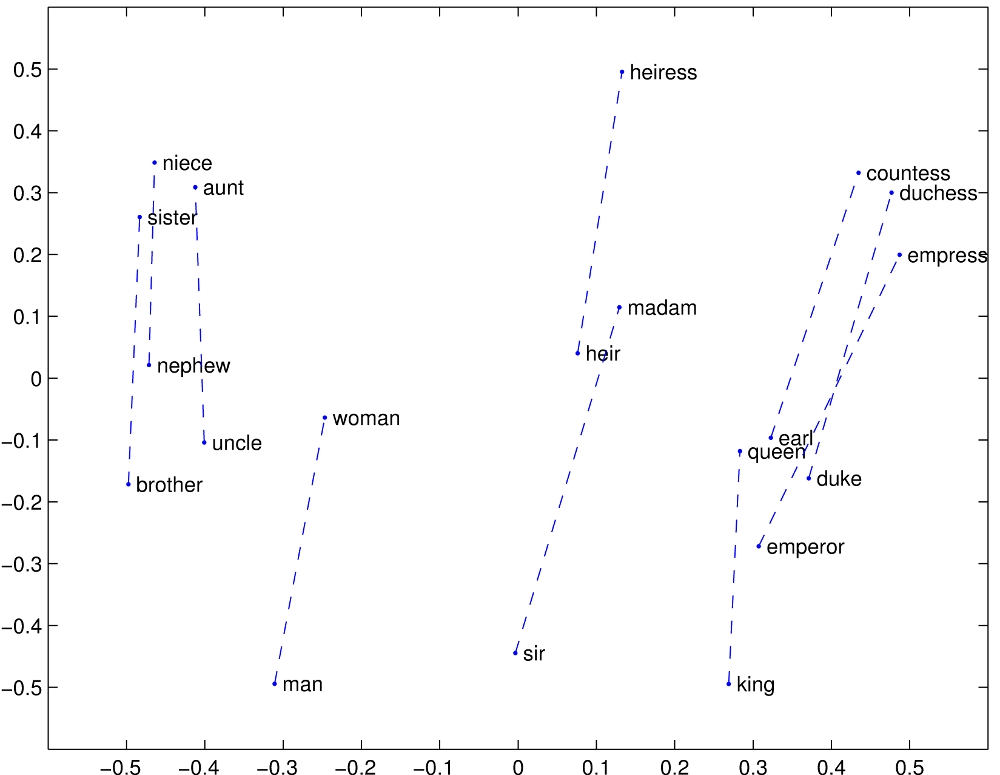
\includegraphics[width=0.8\linewidth]{data/man_woman}
			\caption{Representation of words relating to the differentiation between man and woman}
			\label{fig:wordembeddings}
		\end{figure}
		
		The high dimensional vector representations of the words can be processed with the \textit{t-SNE} dimensionality reduction algorithm to be able to plot them in a two dimensional vector space. Figure \ref{fig:wordembeddings} shows a section of the vector space.
		
		\subsection{POS-Tagging}

		POS-Tagging (part-of-speech tagging), also called grammatical tagging or word-category disambiguation, refers to the process of identifying particular parts of speech like nouns or verbs. 

		Identifying the role of a certain word within a sentence is important for the task of sentiment analysis, as identifying entities and their corresponding aspects can be handled much easier relying on certain assumptions about the part of speech of words.

		Frequent nouns or noun phrases often describe aspects of products and the vocabulary that is used to describe those usually converges. With such an approach many important aspects can easily be found, but on a more general scheme grammatic based relationships can be used to extract important aspects.

		For example words that express opinion on something, like 'great' or 'bad' can be incorporated in rules to extract aspects. To sum it up POS-Tagging is an important part of sentiment analysis.
		
		While being important POS-Tagging is also a complex problem. Word-forms in natural language are often ambiguous. For example the word 'dogs' is usually thought of as a plural noun, but can be used as a verb as well:

		\begin{quote}
			The sailor dogs the hatch.
		\end{quote}

		Due to the complexity, machine learning techniques are often applied in POS-Taggers. Popular approaches such as the Viterbi algorithm, the Brill tagger or the Baum-Welch algorithm work with techniques such as dynamic programming, supervised learning or hidden Markov models.
		
		\subsection{NER-Tagging}
		
		Named-Entity recognition (NER) is a task that seeks to locate and classify specific information in text. This information is called a named entity and can refer to categories such as the names of persons, locations, times or many others.

		An annotated sentence could look like this :

		\begin{quote}
			[Tim Cook]$_{[Person]}$ has a Net worth of [785 million USD]$_{[Monetary Value]}$ as of [March 16. 2017]$_{[Time]}$.
		\end{quote}
		
		Often the task of NER-Tagging is separated into two. In the first part names are detected and in the second part these names are classified. 
		
		While state-of-the-art NER-Taggers perform very well and produce near-human performance they are also brittle and do not perform well in domains they were not designed for.

		\subsection{Dependency parsing}
		
		Dependency parsing is a method of building up context in a sentence.
		It looks on the relations each word has with the other words and tries to create a meaning out of a sentence by that.
		
		For example the sentence \textit{I saw a girl with a telescope} has two times the combination of an object with the word \textit{a}. 
		The word \textit{girl} is specified by the verb \textit{saw} and the object \textit{telescope} is specified by the word \textit{with} with references to the verb \textit{saw}. 
		The verb \textit{saw} relates then to the noun \textit{I} as it is the subject. 		
		A visualization can be seen in the following.
		This is however just one method of analyzing this sentence.
		Another way of seeing this sentence would be to relate the word \textit{with} with the object \textit{girl} which is possible in the language and gives the whole sentence a different meaning.
		
		\begin{figure}[h]
			\centering
			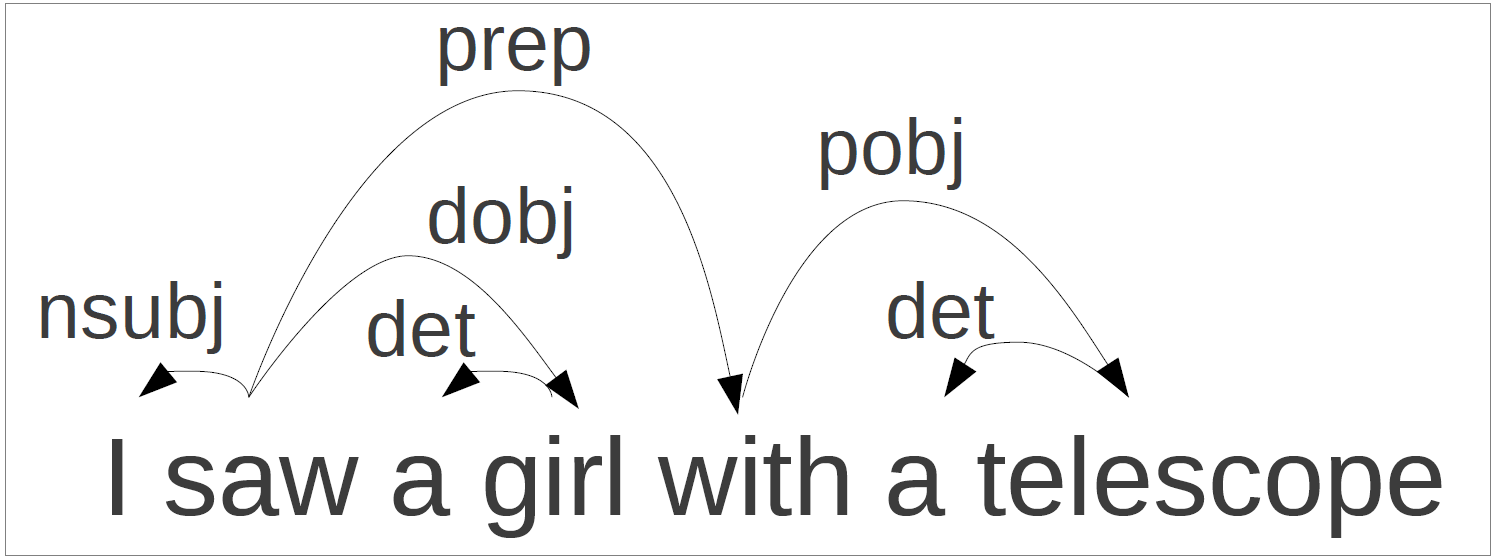
\includegraphics[width=0.8\linewidth]{data/dependency}
			\caption{The dependency parsing example}
			\label{fig:dependency}
		\end{figure}
		
		This example has been taken from \cite{dependency}.
	
	\section{Preprocessing}
	
	We preprocessed the data by extracting the actual text of the posts into separate files, which can be processed by SyntaxNet. We decided to exclude posts that are less than 20 characters long or include images. This is due to the fact that posts which are too short do not yield much information most of the time. Furthermore, posts that include images often refer to objects in the image, which makes it hard to understand the author's sentiment without analyzing the image content.
	
	\section{Co-Reference Resolution}
	
	\section{Extracting entities and aspects}
	\label{sec:extraction}
	To be able to determine the customers' opinions on certain entities and their aspects, we first need to extract possible entities and aspects from the given dataset. For this task, we will use a method proposed by \cite{Hu:2004:MSC:1014052.1014073}, which consists of the following two steps:
	
	First, we identify frequent nouns and noun phrases with a POS-Tagger. Since people commenting on aspects of a product usually use a limited vocabulary, this process should yield a first set of possible entities and aspects. The frequency threshold needs to be chosen experimentally.
	
	However, since the first step can miss quite a lot of important aspects, the next step tries to find some of them by exploiting the relationships between aspects and opinion words.
	
	\section{Determining sentiment polarities}
	For determining the sentiment polarities, we used the Lexicon-based approach which will the describe in the following.
	
		\subsection{Lexicon-based approach}
		An approach to determine sentiment polarities is the lexicon-based approach.
		
		We applied a method by \cite{Ding:2008:HLA:1341531.1341561}, which can be broken down to the following four steps: 
		
		In the first step, all sentiment words and phrases in the text will be marked with the help of a sentiment lexicon. This is done by assigning positive or negative values to those sentiments, e.g. [+1] for a positive or [-1] for a negative sentiment.
		
		In the second step, sentiment shifters will be applied. A sentiment shifter can be described as a word that negates the value that has been applied in the first step, changing its value from positive to negative or the other way around. Typically, these words are negation words like \textit{not}. 
		
		In the third step, but-clauses and further contrary words are handled. With these contrary words, sentences can be split up into two parts. Depending on the value of the sentiments mentioned in the first part, the sentiments in the second part receive the opposite value.
		
		In the fourth and last step, the opinions need to be aggregated according to the following function:
		\begin{displaymath}
			score(a_i,s) = \sum_{ow_j \in s} \frac{sw_j.so}{dist(sw_j,a_i)}
		\end{displaymath}
		where $sw_j$ is a sentiment word in s, $dist(sw_j, a_i)$ is the distance between aspect $a_i$ and sentiment word $sw_j$ in $s$. $sw_j.so$ is the sentiment score of $sw_i$.  Depending on the score, it can be determined whether the opinion on the aspect $a_i$ in $s$ is positive or negative. If the final score neither positive or negative, it is a neutral aspect.
	
		This method can be made more effective by applying dependency parsing to the sentences, such that the scope of each individual sentiment word can be determined more accurately. This allows us to discover the sentiment orientation of context dependent words \cite{Liu12sentimentanalysis}. Due to limited time however this approach was not followed.

	\section{Results}
	
	% Has to be enhanced => NLTK => OpenNLP
	We built and tested the syntax parser \textit{Parsey McParseface} (aka SyntaxNet) by Google, which we used as POS-Tagger for extracting entities and aspects and as dependency parser for several other tasks. SyntaxNet is easy to use and yields state-of-the art results. Moreover, it is based on Google's Deep Learning Framework TensorFlow and therefore integrates nicely into the rest of our implementation. The implemented models are explained in detail in \cite{DBLP:journals/corr/AndorAWSPGPC16}.
	
	
	% Has to be rewritten	
	We will use the sentiment lexicon by \cite{Hu:2004:MSC:1014052.1014073}, which includes mis-spellings, morphological variants, slang and social-media mark-up of 2006 positive and 4783 negative words. Moreover, we will use pre-trained word embeddings from the GloVe project \cite{pennington2014glove}.
	
	\subsection{Visualization}

	\section{Previously defined goals and their fulfillment}
	The overall goal is to extract as many quintuples $(e_i, a_{ij}, s_{ijkl}, h_k, t_l)$ as possible, where $e_i$ is the $i$'th entity and $a_{ij}$ is the $j$'th aspect of entity $i$ the opinion is expressed on. $s_{ijkl}$ is the sentiment polarity, which can take on the values \textit{positive} or \textit{negative}. $h_k$ describes the opinion holder and $t_l$ the time at which the opinion was expressed.
	
	We build a database with opinions and statistics on several products and their aspects. For a visualization of the results we build a simple dashboard with state-of-the-art web technologies.

	Based on these goals the following research questions were defined:

	\begin{itemize}
	\item Do state of the art techniques in sentiment analysis provide valuable results when applied to Facebook posts?
	\item How do supervised (LSTM-Network) and unsupervised (Lexicon-based) techniques for sentiment analysis compare?
		\begin{itemize}
		\item Is it possible to apply the LSTM-Network approach proposed by \cite{hongsentiment} on an aspect level, rather than document level?
		\item Which technique offers better results, how does it compare to the effort required to use that technique?
		\item How does a combination of the techniques affect performance?
		\end{itemize}
	\end{itemize}
	
	
	
	\section{The code pipeline}
	To reproduce our work, the provided code has to be executed in a certain sequence. The following will talk about the needed steps.
	
	\section{Conclusion and Future Work}
	
	\newpage
	
	\nocite{Zhang2014}
	\nocite{syntaxnet}

	\bibliography{rp}
	\bibliographystyle{apacite}
\end{document}